\subsection{Proof of Relay}
\label{sec:incentives:proofofrelay}

The \nameref{sec:sphinx} guarantees that packets can only get processed in the order that has been chosen by the creator. As a result, after applying the required transformations, the next downstream node can either decode the packet or ends up with some random bitstring. Hence it is the next downstream node who is able to verify the correctness of the previously applied transformations which it confirms by sending an acknowledgement.

\begin{figure}[H]
      \centering
      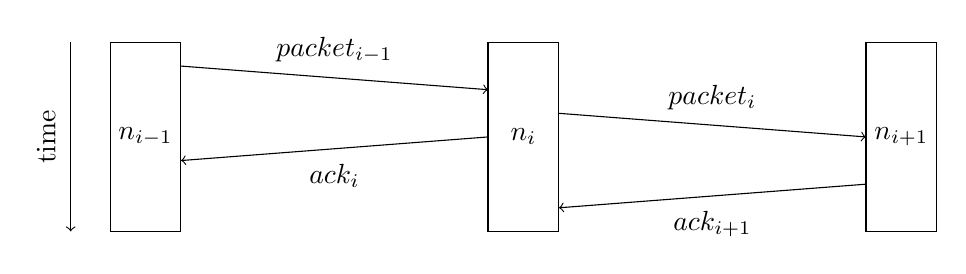
\begin{tikzpicture}
            \def\one{0.6}
            \def\nodeHeight{4*\one}
            \def\nodeWidth{1.5*\one}
            \def\nodeOffset{8*\one}

            \foreach \i\name in{0/$n_{i-1}$,1/$n_i$,2/$n_{i+1}$} {
                        \draw[shift={(\i*\nodeOffset,0)}] (0,0) rectangle (\nodeWidth,-\nodeHeight) node[midway] {\name};
                  }

            \foreach \i\packet\ack in{0/$packet_{i-1}$/$ack_i$,1/$packet_{i}$/$ack_{i+1}$} {
                        \draw[->,shift={(\i*\nodeOffset,-\i*\one)}] (\nodeWidth,-0.5*\one) -- (\nodeOffset,-\one) node[midway,above=2pt] {\packet};

                        \draw[->,shift={(\i*\nodeOffset,-\i*\one)}] (\nodeOffset,-2*\one) -- (\nodeWidth,-2.5*\one) node[midway,below=2pt] {\ack};
                  }

            \draw[->] (-0.5,0) -- (-0.5,-\nodeHeight) node[midway,left=2pt] {\rotatebox{90}{time}};
      \end{tikzpicture}
      \caption{Node $n_{i-1}$ sends $packet_{i-1}$ to node $n_i$. Node $n_i$ transforms the incoming packet, resulting in ${packet_i}$ and sends it to node $n_{i+1}$. Afterwards it acknowledges the processing of $packet_{i-1}$ to node $n_{i-1}.$}
\end{figure}

Note that acknowledgements are sent immediately once the processing of the incoming packet has been completed. This makes sure that sending acknowledgements does not create any observable pattern in reverse to the chosen path. It is rather that each acknowledgement depends on one incoming packet but it does not depend on the chosen path.

\paragraph{Construction}

Each ticket includes a challenge $C_i$ which requires a response $response_i$ to be claimable on-chain. The creator of the packet samples all of them and uses the first one for the ticket sent to the first relayer. All subsequent ones are put into the section of the routing information, see section \ref{sec:sphinx:routinginformation}, that is visible by the corresponding node. Each relayer $n_i$ and their corresponding next downstream node $n_{i+1}$ engage in a 2-out-of-2 secret sharing of $response_i$ picked by the creator of the packet. To convince each relayer that the creator of the packet knows any value $\widetilde{response_i}$ that solves $C_i$, each relayer $n_i$ receives a value $hint_i$ that serves as an argument of knowledge.

\begin{figure}[H]
      \label{fig:packetDetails}
      \centering
      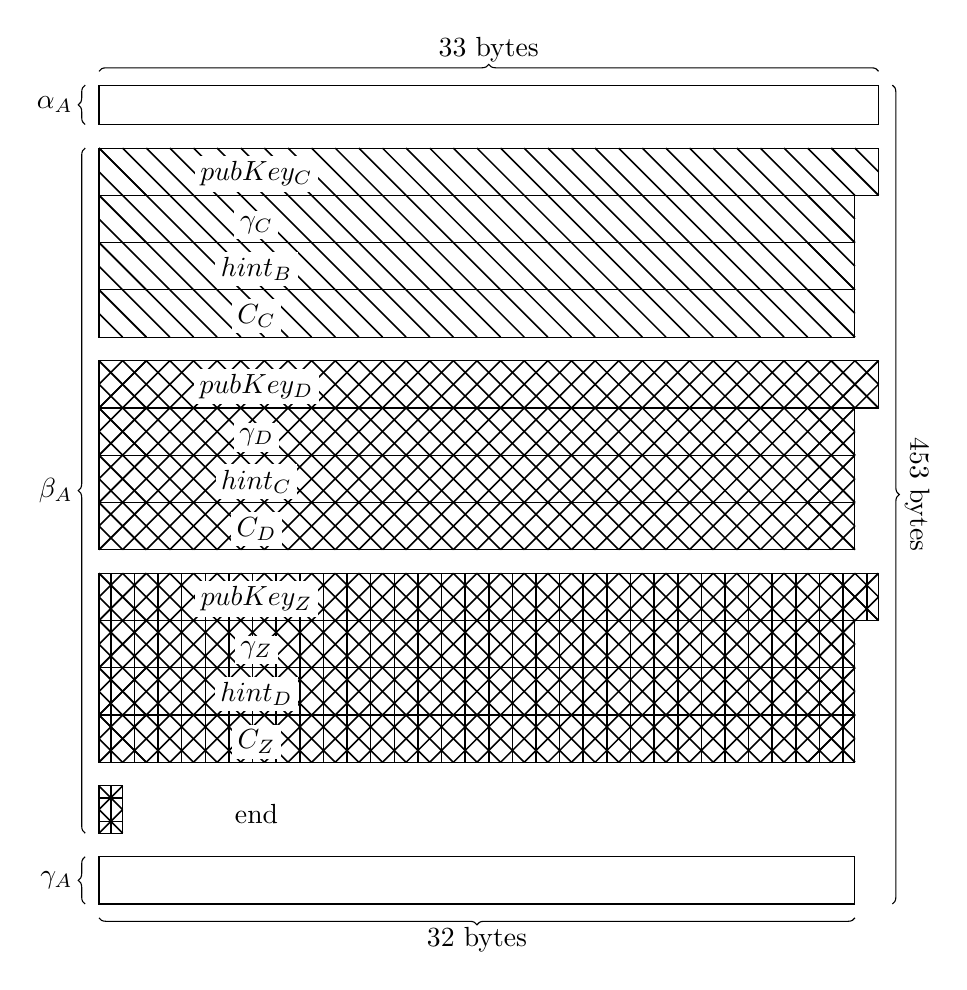
\begin{tikzpicture}
            \def\one{0.3}
            \draw[decoration={brace,raise=5pt},decorate] (0,0.5) -- node[above=5pt] {33 bytes} (33*\one,0.5);
            \draw[decoration={brace,raise=5pt},decorate] (0,0) -- node[left=6pt] {$\alpha_A$} (0,0.5) ;
            \draw[black] (0,0) rectangle (\one*33,0.5);

            \draw[decoration={brace,raise=5pt},decorate] (0,-9.0) -- node[left=6pt] {$\beta_A$} (0,-0.3);

            \foreach \name\length\offset\hatching in{$pubKey_C$/33/-0.9/1,$\gamma_C$/32/-1.5/1,$hint_B$/32/-2.1/1,$C_C$/32/-2.7/1,$pubKey_D$/33/-3.6/2,$\gamma_D$/32/-4.2/2,$hint_C$/32/-4.8/2,$C_D$/32/-5.4/2,$pubKey_Z$/33/-6.3/3,$\gamma_Z$/32/-6.9/3,$hint_D$/32/-7.5/3,$C_Z$/32/-8.1/3}{
                        \draw (0,\offset) rectangle (\one*\length,\offset+0.6);
                        \begin{scope}[shift={(0,\offset)}]
                              \ifnum\length=33
                                    \def\a{9.9}
                                    \def\diff{9.4}
                              \else
                                    \def\a{9.6}
                                    \def\diff{9.1}
                              \fi
                              \def\b{0.6}
                              \def\lw{0.2}

                              \foreach \x [count=\i] in{0,0.3,0.6,...,\b}{
                                          \draw [line width=\lw mm](\x,0)--(0,\x) (\a-\b+\x,\b)--(\a,\x);
                                    }
                              \foreach \x [count=\i] in{0,0.3,0.6,...,\diff}{
                                          \draw [line width=\lw mm](\x+\b,0)--(\x,\b);
                                    }

                              \ifnum\hatching>1
                                    \foreach \x [count=\i] in{0,0.3,0.6,...,\b}{
                                                \draw [line width=\lw mm](0,\x)--(\b-\x,\b) (\a-\b+\x,0)--(\a,\b-\x);
                                          }
                                    \foreach \x [count=\i] in{0,0.3,0.6,...,\diff}{
                                                \draw [line width=\lw mm](\x,0)--(\b+\x,\b);
                                          }
                              \fi

                              \ifnum\hatching>2
                                    \foreach \x [count=\i] in{0,0.15,0.45,...,\a}{
                                                \draw [line width=\lw mm](\x,0)--(\x,\b);
                                          }
                              \fi
                        \end{scope}

                        \draw (2.0,\offset+0.25) node[fill=white,above=-6pt,inner sep=2pt] {\name};
                  }

            \draw (0,-8.4) rectangle (\one*1,-9.0);

            \begin{scope}[shift={(0,-9.0)}]
                  \def\lw{0.2}

                  \draw [line width=\lw mm](0,0)--(0.3,0.3);
                  \draw [line width=\lw mm](0,0.3)--(0.3,0.6);

                  \draw [line width=\lw mm](0,0.6)--(0.3,0.3);
                  \draw [line width=\lw mm](0,0.3)--(0.3,0);

                  \draw [line width=\lw mm](0.15,0)--(0.15,0.6);

                  \draw [line width=\lw mm](0,0.15)--(0.3,0.15);
                  \draw [line width=\lw mm](0,0.45)--(0.3,0.45);

                  \draw (2.0,0.25) node[fill=white,above=-7pt] {end};
            \end{scope}

            \draw[decoration={brace,raise=5pt},decorate] (0,-9.9) -- node[left=6pt] {$\gamma_A$} (0,-9.3);

            \draw (0,-9.3) rectangle (\one*32,-9.9);
            \draw[decoration={brace,mirror,raise=5pt},decorate] (0,-9.9) -- node[below=5pt] {32 bytes} (32*\one,-9.9);

            \draw[decoration={brace,raise=5pt},decorate] (33*\one,0.5) -- node[midway,right=6pt] {\rotatebox{270}{453 bytes}} (33*\one,-9.9) ;

      \end{tikzpicture}
      \caption{Mixnet packet header with PoR fields that is sent from the sender $A$ to $B$ and supposed to be forwarded through nodes $C, D$ to $Z$.}
\end{figure}

\paragraph{Secret sharing}
\label{sec:incentives:proofofrelay:secretSharing}

Each node derives two keys, $s_i^{own}$ and $s_i^{ack}$, by using the $s_i$ as given by the SPHINX packet (see the \lcnameref{appendix:keyderivation} section for more details). $s_i^{own}$ and $s_{i+1}^{ack}$ serve as key shares of a 2-out-of-2 secret sharing between a node $n_i$ and the next downstream node $n_{i+1}$ along the chosen path. Once a node knows \textit{both} key shares, $s_i^{own}$ and $s_{i+1}^{ack}$, it is able to reconstruct $s_i^{response}$ to redeem the received ticket on-chain.

Whilst $s_i^{own}$ is derivable upon reception of a packet, $s_{i+1}^{ack}$ requires the cooperation of the next downstream node $n_{i+1}$ and is sent as an \textit{acknowledgement} if $n_{i+1}$ has received the transformed packet and considers both the packet and embedded ticket valid.

\begin{figure}[H]
      \centering
      \begin{tikzpicture}[auto]
            \draw (0,0) node (a) {};
            \draw (3.0,0) node (b) [rectangle,draw] {$n_{i-1}$};
            \draw (6,0) node (c) [rectangle,draw] {$n_i$};
            \draw (9.0,0) node (d) [rectangle,draw] {$n_{i+1}$};
            \draw (12.0,0) node (e) {};

            \draw (6.0, -1.5) node [circle,draw] (intermediateResult) {};
            \draw (6.0, -2.5) node (response) {$s_i^{response}$};

            \draw [->,draw,dashed] (a.east) to node [align=center,below] {packet$_{i-2}$} (b.west);
            \draw [->,draw,dashed] (b.east) to node [align=center,below] {packet$_{i-1}$} node [align=center,above,circle] {\color{hopr-blue}1.} (c.west);
            \draw [->,draw,dashed] (c.east) to node [align=center,below] {packet$_i$} node [align=center,above,circle] {\color{hopr-blue}2.} (d.west);
            \draw [->,draw,dashed] (d.east) to node [align=center,below] {packet$_{i+1}$} (e.west);

            \draw [->,draw] (c.south) to node [right] {$s_i^{own}$} node [align=center,left=1pt,circle] {\color{hopr-blue}3.}  (intermediateResult.north);
            \draw [->,draw,bend left] (d.south) to node[below] {$s_{i+1}^{ack}$} node [align=center,right=5pt,circle] {\color{hopr-blue}4.} (intermediateResult.east);
            \draw [->,draw] (intermediateResult.south) to (response.north);
      \end{tikzpicture}
      \caption{\color{hopr-blue}1. \color{black} Node $n_i$ receives $packet_{i-1}$, validates it, transforms it and \color{hopr-blue}2. \color{black} sends it to node $n_{i+1}$. \color{hopr-blue}3. \color{black} While processing $packet_i$, node $n_i$ derives $s_i^{own}$ and \color{hopr-blue}1. \color{black} once node $n_{i+1}$ considers $packet_i$ valid, it \textit{acknowledges} the receipt of $packet_i$ and thereby reveals $s_{i+1}^{ack}$ to node $n_i$ which allows node $n_i$ to reconstruct $s_i^{response}$.}
      \label{fig:proofofrelay}
\end{figure}

\paragraph{Challenge response}

Tickets sent next to a mixnet packet include a challenge $C_i$ which is computed as $$C_i = s_i^{response} \cdot G = (s_i^{own} + s_{i+1}^{ack}) \cdot G$$ where $G$ refers to the base point and $\cdot$ means scalar multiplication on the curve. Hence, in order to solve the challenge, it is necessary to know $s_i^{own}$ as well as $s_{i+1}^{ack}$.

\paragraph{Challenge and Hint}
\label{sec:incentives:proofofrelay:challenge}

Once a node receives a packet, it is able to derive $s_i^{own}$ but it is unable to decide whether $s_{i+i}^{ack}$ will ever lead to $s_i^{response}$ that solves the challenge. Since the underlying field preserves the distributivity, it holds that $$C_i = s_i^{response} \cdot G = (s_i^{own} + s_{i+1}^{ack}) \cdot G = s_i^{own} \cdot G + s_{i+1}^{ack} \cdot G$$

Hence by knowing $hint_i = s_{i+1}^{ack} \cdot G$, the node can verify that $s_i^{own} \cdot G + hint_i = C_i$ and thereby check that the creator of the challenge must have known a value $\tilde{s}_{i+1}^{ack}$ that led to $hint_i$. Due to the infeasibility of inverting scalar multiplication on the chosen curve, knowing $hint_i$ does not reveal $s_{i+1}^{ack}$. Hence, by embedding $hint_i$ into the part of $\beta$ within the SPHINX packet that is readable by node $n_i$, the sender makes the validity of the embedded challenge verifiable.

As the next downstream node would not accept a packet without a ticket\footnote{By default, nodes only forward packets that include incentives. Nevertheless, the protocol does not prevent them from processing packets without enforcing an incentive.}, the node $n_i$ not only needs to transform the packet but must also issue a ticket to the next downstream node $n_{i+1}$. Therefore, it needs to know which challenge $\tilde{C}_{i+1}$ to put into the ticket issued for node $n_{i+1}$. As in the previous section, this is done with the help of the creator of the packet, who embeds $C_{i+1}$ into the part of the SPHINX packet that is readable by node $n_{i+1}$.

By chaining this principle, nodes are forced to \textit{always} issue a ticket to the next downstream node because they are unable to claim their own incentive without the help of the next downstream node.

Since the very last node, namely the final recipient, of the packet, does not need to forward the packet to anyone else, it has no direct incentive to acknowledge tickets, hence there are no direct consequences for not acknowledging packet. In its current version, the protocol does not prevent this kind of behaviour, but research is being conducted into the necessity and feasibility of solving this issue via a reputation system.